\chapter{Om Kojo}
\begin{multicols}{2}
\section*{\color{black}Vad är Kojo?}
Kojo är en app som hjälper dig att lära dig att programmera. Med Kojo kan du koda i det moderna och kraftfulla programspråket Scala. Kojo är gratis och finns på Svenska. Kojo fungerar med Linux, Windows och Mac OSX.
\section*{\color{black}Var hittar jag Kojo?}
Ladda ner Kojo här: 
\href{http://www.kogics.net/kojo-download}{www.kogics.net/kojo-download}
Läs mer här: 
\href{http://lth.se/programmera}{lth.se/programmera}

\columnbreak

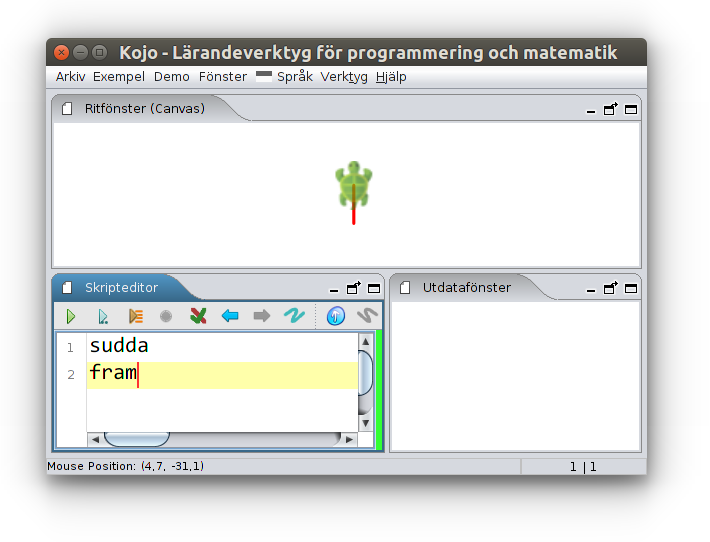
\includegraphics[width=14cm]{../img/kojo.png}
\end{multicols}

\chapter{Ditt första program}
\begin{multicols}{2}
\section*{\color{MidnightBlue}Du lär dig att:}
Skriva kod i en editor.\\
Köra igång ett program.
\section*{\color{BrickRed}Uppdrag:}
Skriv detta program i editorn:

\begin{lstlisting}[basicstyle={\ttfamily\fontsize{24}{24}\selectfont}]
sudda
fram
\end{lstlisting}
        
Tryck på den gröna play-knappen\\
för att köra igång ditt program.

\columnbreak

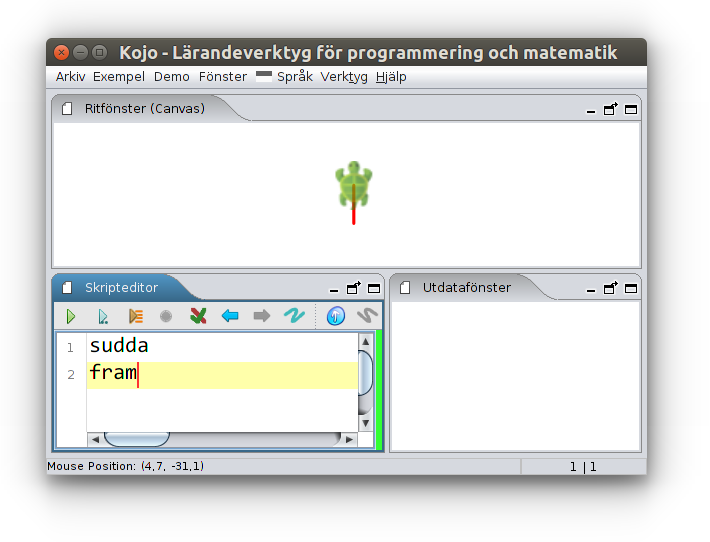
\includegraphics[width=14cm]{../img/fram.png}
\end{multicols}

\chapter{Rita en kvadrat}
\begin{multicols}{2}
\section*{\color{MidnightBlue}Du lär dig att:}
Satser i sekvens görs i tur och ordning.\\
Ordningen spelar stor roll.
\section*{\color{BrickRed}Uppdrag:}
Skriv in och utöka detta program så att paddan ritar en kvadrat:

\begin{lstlisting}[basicstyle={\ttfamily\fontsize{24}{24}\selectfont}]
sudda
fram
höger
\end{lstlisting}
        

\columnbreak

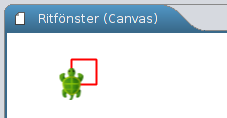
\includegraphics[width=14cm]{../img/kvadrat.png}
\end{multicols}

